\let\textcircled=\pgftextcircled
\chapter{Introduction}
\label{chap:intro}

\initial{K}ey to autonomy is the concept of self, and awareness of how ones self fits into the surrounding environment. For an autonomous robot this is largely encompassed by position and orientation as well as movement relative to the surroundings, collectively referred to as the state of the robot. This information is vital for enabling the robot to operate unhindered and without incident. Drones are a versatile platform as their access to a third dimension while maintaining the ability to hold stationary (unlike a fixed wing aircraft) means that they can be deployed in many environments with a wide variety of uses. This does come at the cost of needing to have even greater accuracy with regards to pathing and collision avoidance. Use cases for drones include aerial mapping and photography, surveillance, package delivery and scientific research in hostile environments. \par
	The highly accurate sensory apparatus often required for this kind of navigation can be very expensive, hence a smarter method of sensory integration allowing use of cheaper apparatus could cut back on a lot of the cost. This project will compare a variety of cheap sensors to develop an appropriate suite capable of precise data production. Following that a form of sensor fusion will be applied to the sensory suite as well as any other gleanable information to provide accurate state estimates. \par
    The drone itself is based on a HobbyKing\textsuperscript{TM} S550 hexcopter frame \cite{hobbyking2016s550} with parts:
\begin{itemize}
\item Turnigy 4000mAh 4S 40C Lipo Pack
\item AfroFlight Naze32 Rev6 Controller
\item 2-6s 30 Amp BL Heli ESCs
\item EMAX MT2216-810KV brushless motors
\item 10x4.5 CW/CCW propellers
\end{itemize}

and was assembled as part of the project.
\bigskip


Previous work by Santana \textit{et al.} looks to accomplish similar results to this project albeit at a smaller scale with much reduced sensory apparatus \cite{santana2014trajectory}.
	Another paper by Yang \textit{et al.} shows use of the extended Kalman filter (a non-linear Kalman filter variant) to successfully land a multi-sensor rotary-wing unmanned aerial vehicle on a moving ship deck, detailing the use of low cost sensors with limited computational power \cite{yang2011multi}. \par
    
	The following paper presents the use of the Kalman filter on a sensory array that is larger than most examples seen in relevant papers but which is also cost efficient. It strives to achieve high quality results from lower quality components to facilitate the goals outlined above. Discussed also is the choice of sensory apparatus, the workings of the Kalman filter, the non-linear filter variants including why they're unsuitable, and testing procedure. \par
    Paper copies of this thesis include an attached CD containing the program code described in the appendices. 









% %=======
% \section{Section}
% \label{sec:sec01}

% Begins a section.

% \subsection{Subsection}
% \label{subsec:subsec01}

% Begins a subsection.

% %A figures matrix.
% \begin{figure}
% \centering
% \begin{minipage}{3.3cm}
%     \centering
%     \subtop[]{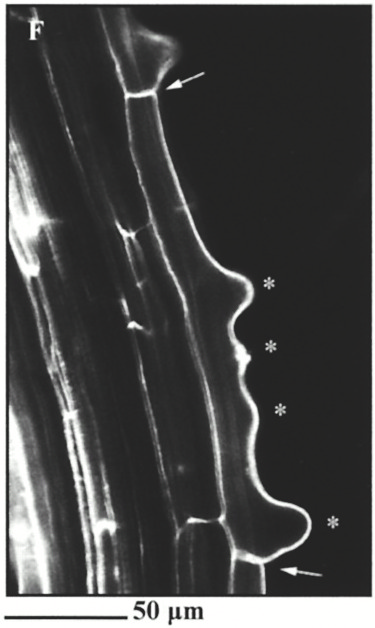
\includegraphics[height=0.28\textheight]{fig01/Nswellings}\label{sf:multiRH02a}}
% \end{minipage}
% \hspace{0.5cm}
% \begin{minipage}{3.3cm}
%     \centering
%     \subtop[]{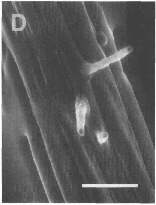
\includegraphics[height=0.27\textheight]{fig01/Mswellings}\label{sf:multiRH02b}}
% \end{minipage}
% \hspace{1.3cm}
% \begin{minipage}{3.3cm}
%     \centering
%     \subtop[]{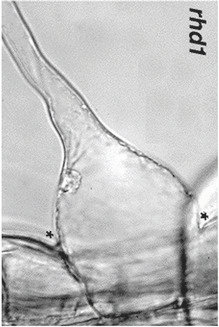
\includegraphics[height=0.27\textheight]{fig01/rhd1}\label{sf:multiRH02c}}
% \end{minipage}
% \\ \vspace{0.1cm}
% \begin{minipage}{10cm}
%     \centering
%     \subtop[]{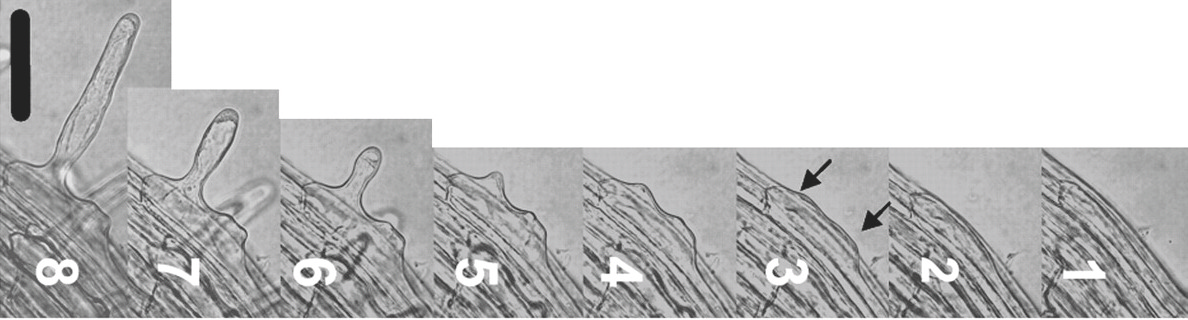
\includegraphics[height=0.145\textheight]{fig01/mutantrhd6}\label{sf:multiRH02d}}
% \end{minipage}
% \\ \vspace{0.1cm}
% \begin{minipage}{10cm}
%     \centering
%     \subtop[]{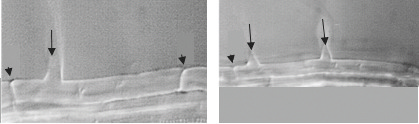
\includegraphics[height=0.16\textheight]{fig01/auxab}\label{sf:multiRH02e}}
% \end{minipage}
% \mycaption[Hair-forming mutant cells.]{(a) A mutant RH cell. Asterisks show multiple sites of RH initiation in a single root hair cell (indicated by the arrows). Figure reproduced from \cite{rigas01}. (b)~Hair-forming cell with three RH initiation locations. The bar represents $50\mu m$. Figure reproduced from \cite{massuci01}. (c) Large bump in mutant {\itshape rhd1}. Figure reproduced from \cite{griersonRH}. (d) Mutant overexpressing gene {\itshape ROP2}; from right-hand to left-hand, numbers indicate progressive snapshots at different times. RH initiation sites are indicated by the arrows. The bar represents $75\mu m$. Figure reproduced from~\cite{mjones01}. (e)~Mutants affected by auxin. On the left-hand side, RH site is farther away from the apical end (left arrow cap); on the right-hand side, multiple RH locations (arrows). Figure reproduced from~\cite{payne01}.}
% \label{fig:multiRH02}
% \end{figure}

% % A single figure
% \begin{figure}[t!]
% 	\centering
% 	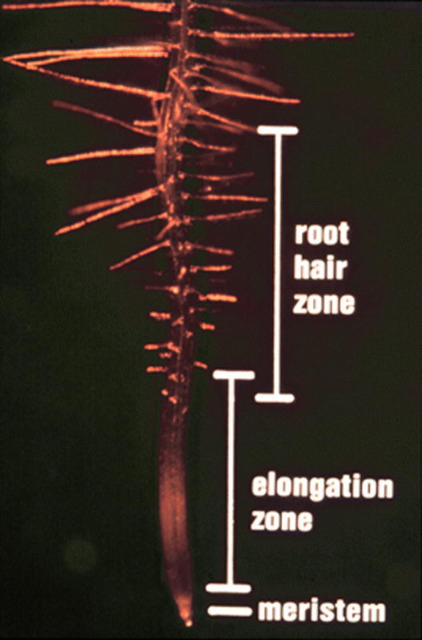
\includegraphics[height=0.35\textheight]{fig01/devepzones}
% 	\mycaption[Developmental zones of an Arabidopsis root.]{Developmental zones of an Arabidopsis root. Figure reproduced from \cite{griersonRH}.}
% 	\label{fig:RHP02}
% \end{figure}


% %=========================================================